% Provenance (never printed): cycle 2 "Questionner l'espace et le temps"
% (oceans, seas, continents on the globe) and "Questionner le monde de la
% matiere" (states of water in natural phenomena); see sources/book1/PROVENANCE.md.
% Book 1, grade 2, chapter 1.
\chapter{L'eau sur la Terre}\label{ch:g2:water-on-earth}

Le 7 décembre 1972, trois astronautes en route vers la Lune ont tourné
leur appareil photo vers la Terre. Leur photographie est devenue l'une des
images les plus célèbres jamais prises. Regarde-la. Tu y vois des nuages
blancs, un peu de terre brune et jaune, la glace blanche en bas --- et du
bleu, du bleu partout. Vue de l'espace, notre planète est une planète bleue.

\begin{omfigure}
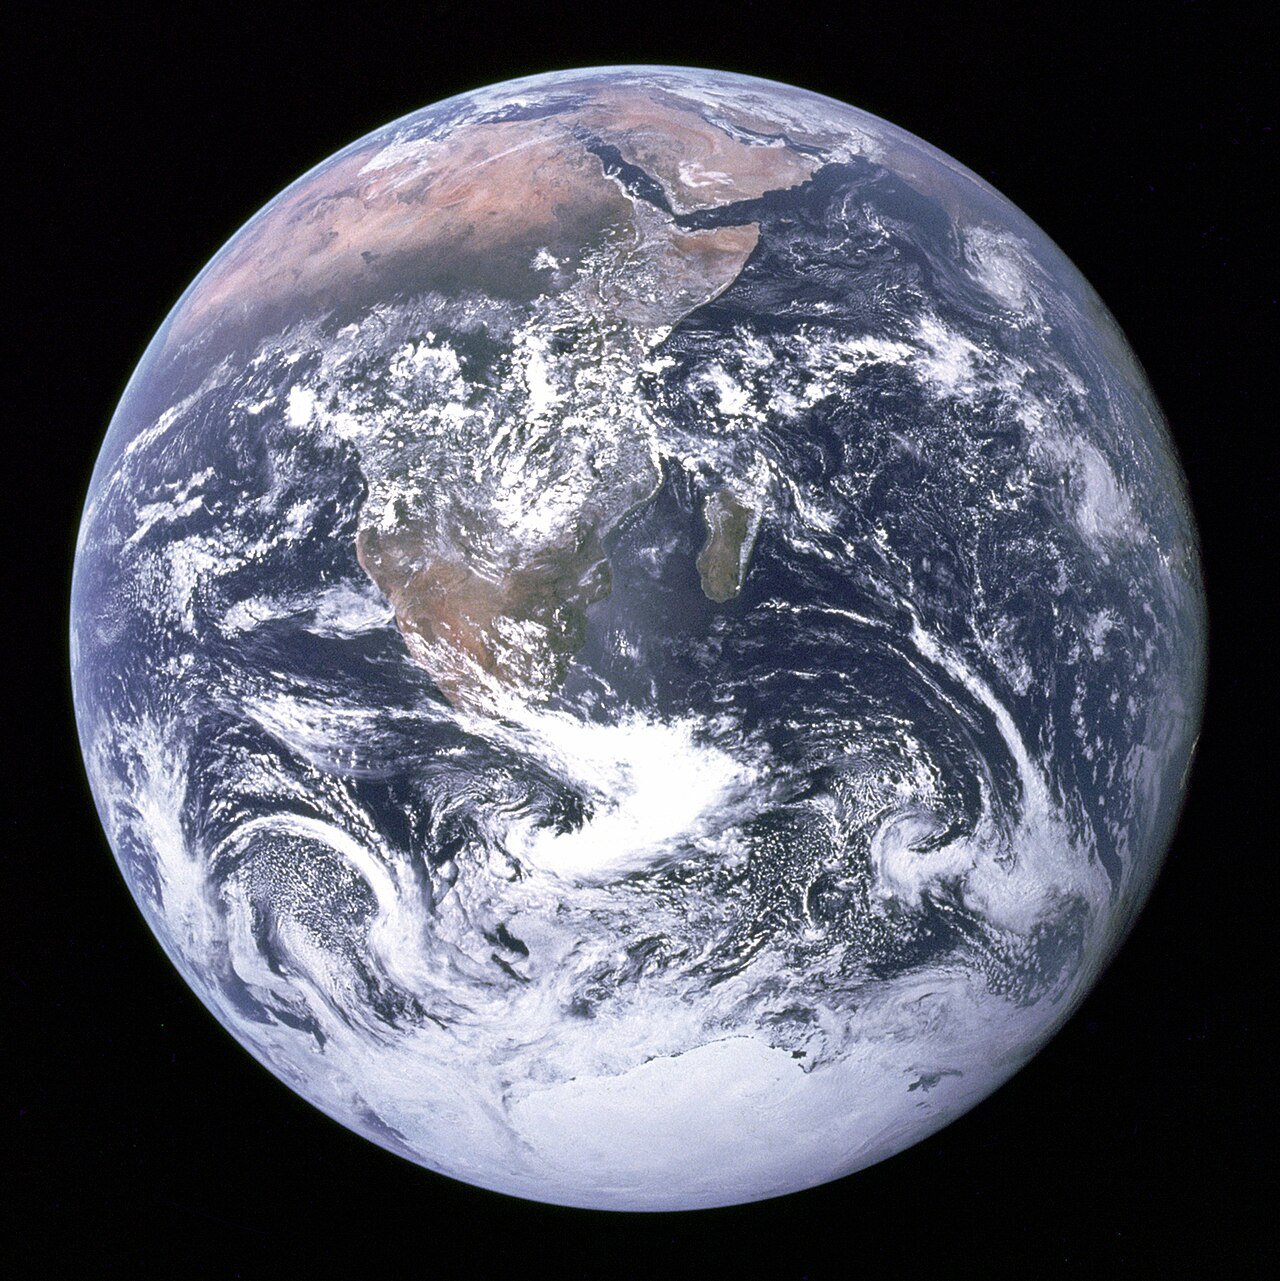
\includegraphics[width=0.5\linewidth]{images/book1/g2-nasa-blue-marble.jpg}

{\small La Terre photographiée par l'équipage d'Apollo~17, le 7~décembre
1972. On voit l'Afrique, l'Arabie en haut, et la glace de l'Antarctique en
bas. Photographie~: NASA (domaine public).}
\end{omfigure}

\begin{recall}
L'eau peut être solide (la glace), liquide, ou un gaz que nous ne voyons
pas (la vapeur d'eau). De l'eau liquide laissée au soleil se change
lentement en vapeur~: elle s'évapore. Quand la vapeur se refroidit, elle
redevient de minuscules gouttes~: elle se condense. Tu as rencontré ces
changements dans les livres de physique. Dans un \omterm{def:g1:landscapes-around-us:landscape}{paysage}, l'eau coule dans
les \omterm{def:g1:landscapes-around-us:water}{rivières} et repose dans les \omterm{def:g1:landscapes-around-us:water}{lacs} (\cref{ch:g1:landscapes-around-us}).
\end{recall}

\section{La planète bleue}

La plus grande partie de la Terre est couverte d'eau. Imagine toute la
surface de la Terre découpée en 100 carrés égaux. Si nous colorions en bleu
chaque carré couvert par la \omterm{def:g2:water-on-earth:ocean}{mer}, nous en colorions 71. Seuls 29 carrés sont
des terres.

\begin{omfigure}
\begin{tikzpicture}
  \begin{axis}[hide axis, width=7.2cm, height=7.2cm, xmin=-0.5, xmax=9.5,
      ymin=-0.5, ymax=9.5, axis equal image, scale only axis,
      clip=false]
    \addplot[scatter, only marks, mark=square*, mark size=9.2pt,
      scatter/classes={0={fill=green!45!omLithAlluv, draw=black!40},
                       1={fill=omSea!80!blue, draw=black!40}},
      point meta=explicit symbolic]
      table[x=col, y=row, meta=blue] {figdata/out/grade-2-ocean_fraction-grid.dat};
  \end{axis}
\end{tikzpicture}

{\small Si la surface de la Terre était découpée en 100 carrés égaux, 71
seraient de la \omterm{def:g2:water-on-earth:ocean}{mer} (en bleu) et 29 des terres (en vert). Calculé à partir
d'une carte du relief de toute la Terre (NOAA ETOPO1).}
\label{fig:g2:water-on-earth:grid}
\end{omfigure}
% ledger: data:etopo1, wss:ocean-cover (71 % computed in figdata/grade-2/ocean_fraction.py)

Les grandes étendues d'\omterm{def:g2:water-on-earth:salt-fresh}{eau salée} qui couvrent la plus grande partie de la Terre portent des noms.

\begin{definition}[Océan et mer]\label{def:g2:water-on-earth:ocean}
Un \emph{océan}\index{ocean@océan} est l'une des très grandes étendues
d'\omterm{def:g2:water-on-earth:salt-fresh}{eau salée} qui couvrent la plus grande partie de la Terre et s'étendent
entre les continents. Une \emph{mer}\index{mer} est une étendue d'\omterm{def:g2:water-on-earth:salt-fresh}{eau
salée} plus petite, en général au bord d'un océan et en partie entourée
de terres.
\end{definition}

Tous les \omterm{def:g2:water-on-earth:ocean}{océans} communiquent entre eux~: un bateau pourrait naviguer de
n'importe quel \omterm{def:g2:water-on-earth:ocean}{océan} à n'importe quel autre sans traverser de terre. Leurs
noms, et leur place sur un globe, sont au \cref{ch:g3:continents-and-oceans}.

\begin{omfigure}
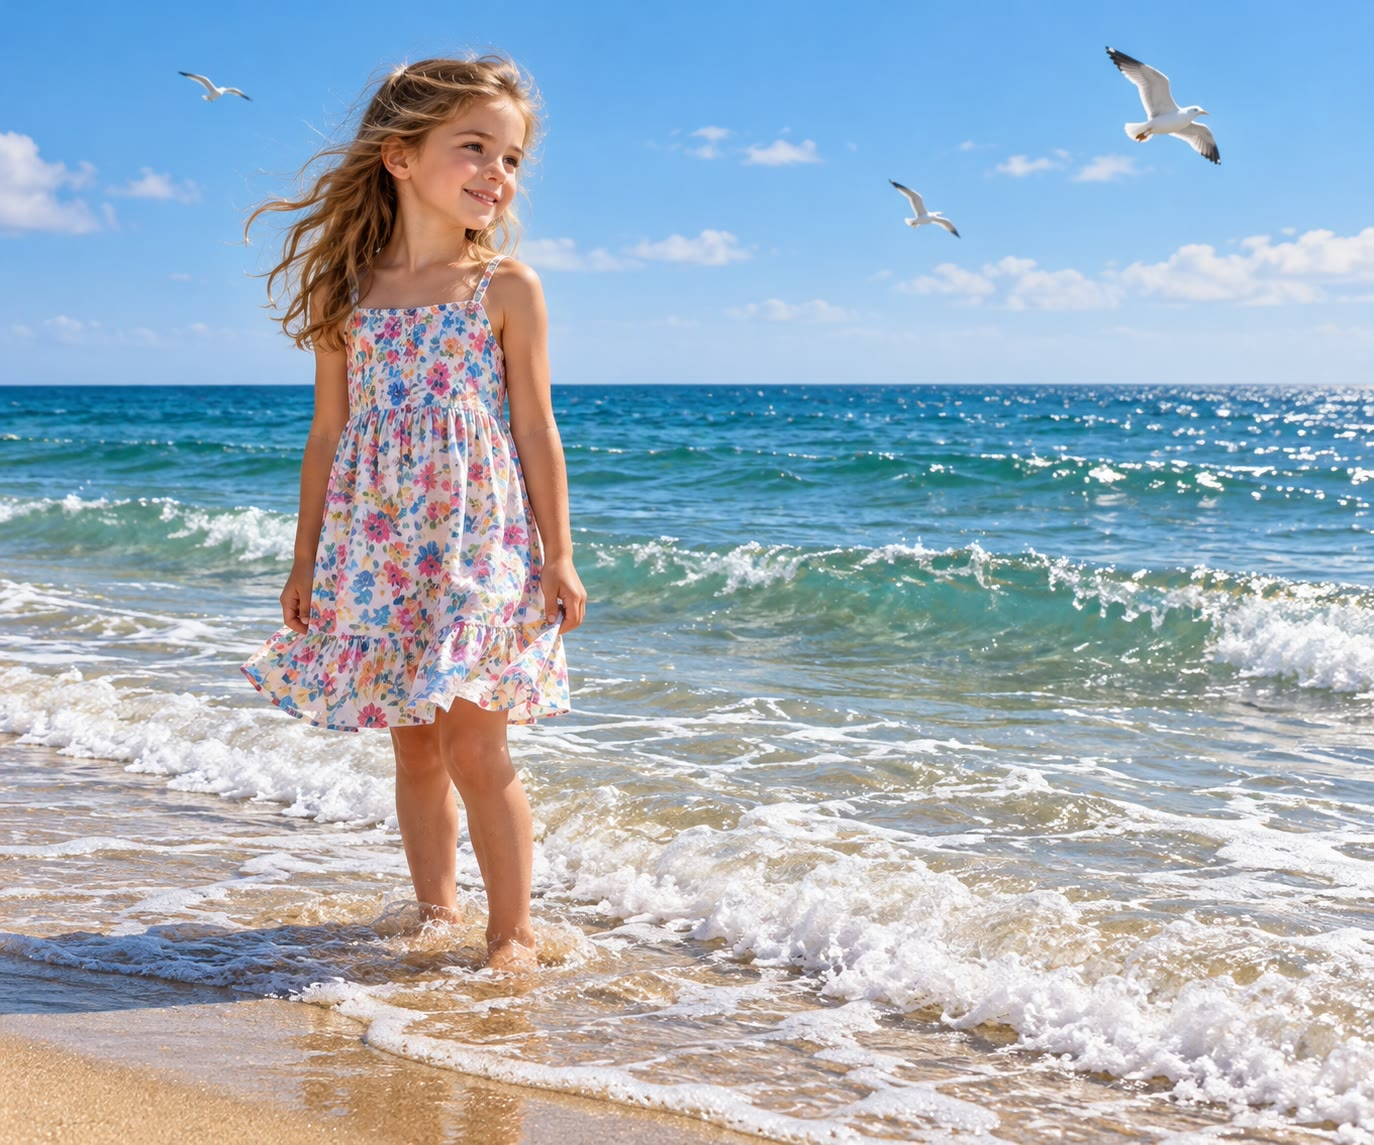
\includegraphics[width=0.62\linewidth]{images/book1/ai/g2-beach-sea.jpg}

{\small Au bord de la \omterm{def:g2:water-on-earth:ocean}{mer}. L'eau continue, bien plus loin que l'œil ne
peut voir.}
\end{omfigure}

\section{L'eau salée et l'eau douce}

Si tu as déjà avalé une gorgée d'eau de \omterm{def:g2:water-on-earth:ocean}{mer} en nageant, tu le sais~: elle
a un goût très salé. L'eau des \omterm{def:g1:landscapes-around-us:water}{rivières} et des \omterm{def:g1:landscapes-around-us:water}{lacs}, non.

\begin{definition}[Eau salée et eau douce]\label{def:g2:water-on-earth:salt-fresh}
L'\emph{eau salée}\index{eau salee@eau salée} contient beaucoup de sel
dissous~: c'est l'eau des \omterm{def:g2:water-on-earth:ocean}{océans} et des \omterm{def:g2:water-on-earth:ocean}{mers}. L'\emph{eau douce}\index{eau douce}
contient très peu de sel~: c'est l'eau de pluie, celle de la plupart des
\omterm{def:g1:landscapes-around-us:water}{rivières} et des \omterm{def:g1:landscapes-around-us:water}{lacs}, de la glace et de la neige, et des sources.
\end{definition}

\begin{example}[La mer est-elle très salée~?]\label{ex:g2:water-on-earth:salty}
% ledger: nos:salinity
Dans une bouteille qui contient un kilogramme d'eau de \omterm{def:g2:water-on-earth:ocean}{mer} --- environ un
litre ---, il y a environ 35 grammes de sel. Si nous laissons toute l'eau
s'évaporer, le sel reste au fond, en cristaux blancs. C'est ainsi que l'on
fabrique le sel de \omterm{def:g2:water-on-earth:ocean}{mer} dans les marais salants, au bord de la \omterm{def:g2:water-on-earth:ocean}{mer}, où le
soleil et le vent assèchent lentement des bassins peu profonds remplis
d'eau de \omterm{def:g2:water-on-earth:ocean}{mer}.
\end{example}

\begin{omfigure}
\begin{minipage}[b]{0.49\linewidth}\centering
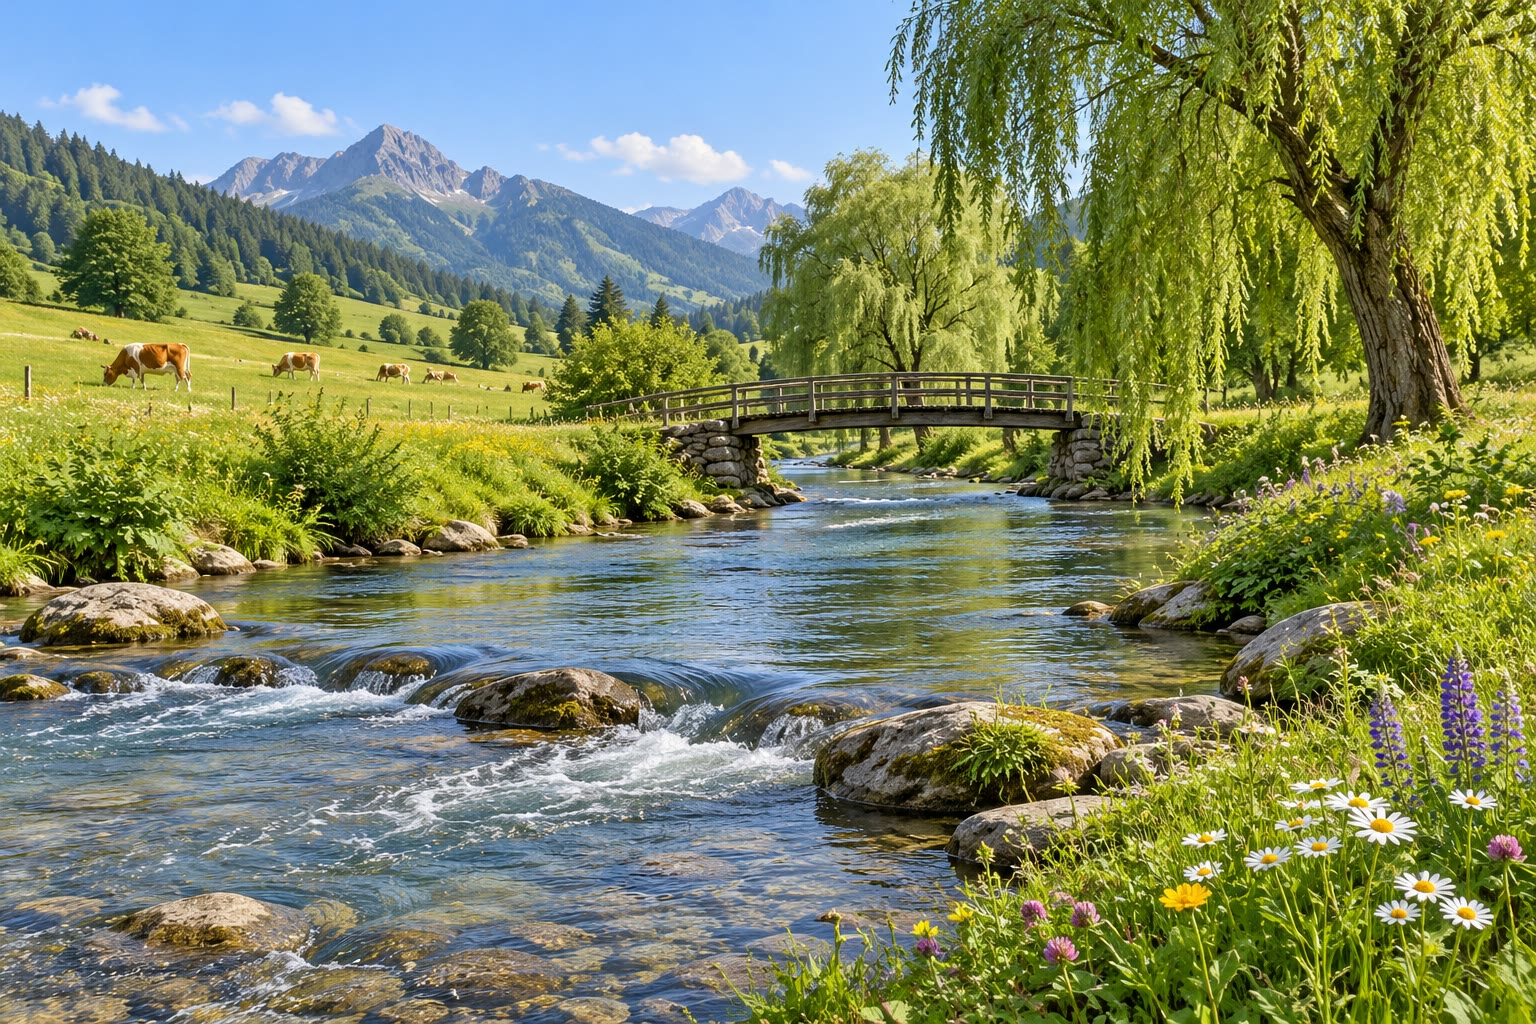
\includegraphics[width=\linewidth]{images/book1/ai/g2-river-meadow.jpg}

{\small De l'\omterm{def:g2:water-on-earth:salt-fresh}{eau douce}~: une \omterm{def:g1:landscapes-around-us:water}{rivière}.}
\end{minipage}\hfill
\begin{minipage}[b]{0.49\linewidth}\centering
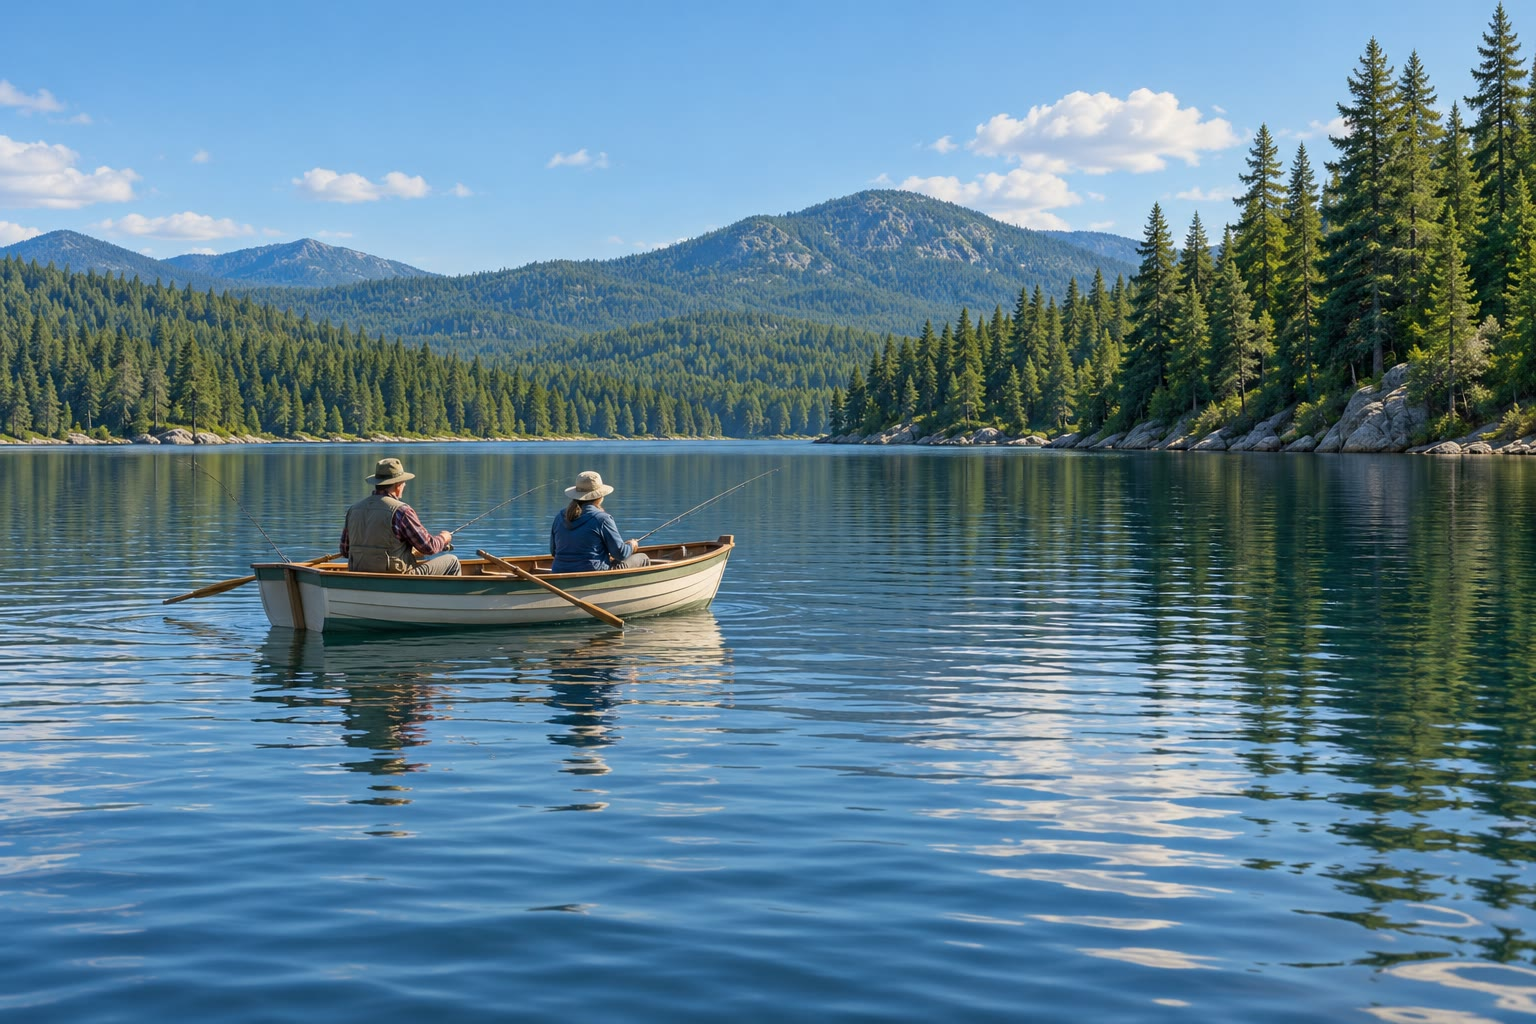
\includegraphics[width=\linewidth]{images/book1/ai/g2-lake-boat.jpg}

{\small De l'\omterm{def:g2:water-on-earth:salt-fresh}{eau douce}~: un \omterm{def:g1:landscapes-around-us:water}{lac}.}
\end{minipage}
\end{omfigure}

\begin{remark}[Nous ne pouvons pas boire l'eau de mer]\label{rem:g2:water-on-earth:drink}
Les êtres humains et les animaux terrestres ne peuvent pas boire l'eau de
\omterm{def:g2:water-on-earth:ocean}{mer}~: elle contient trop de sel, et la boire fait perdre de l'eau au corps
au lieu de lui en apporter. Les marins, loin au large, entourés d'eau, ont
toujours dû emporter leur \omterm{def:g2:water-on-earth:salt-fresh}{eau douce} avec eux.
\end{remark}

\section{Où se trouve toute l'eau~?}

L'\omterm{def:g2:water-on-earth:salt-fresh}{eau douce} n'est pas seulement dans les \omterm{def:g1:landscapes-around-us:water}{rivières} et les \omterm{def:g1:landscapes-around-us:water}{lacs}. Une grande
partie est gelée~: dans les immenses glaces blanches de l'Antarctique et du
Groenland, et sur les hautes \omterm{def:g1:landscapes-around-us:landform}{montagnes}. Une autre grande partie est cachée
sous nos pieds, dans le sol, où elle remplit les minuscules espaces entre
les grains de sable et les fissures de la roche.

\begin{omfigure}
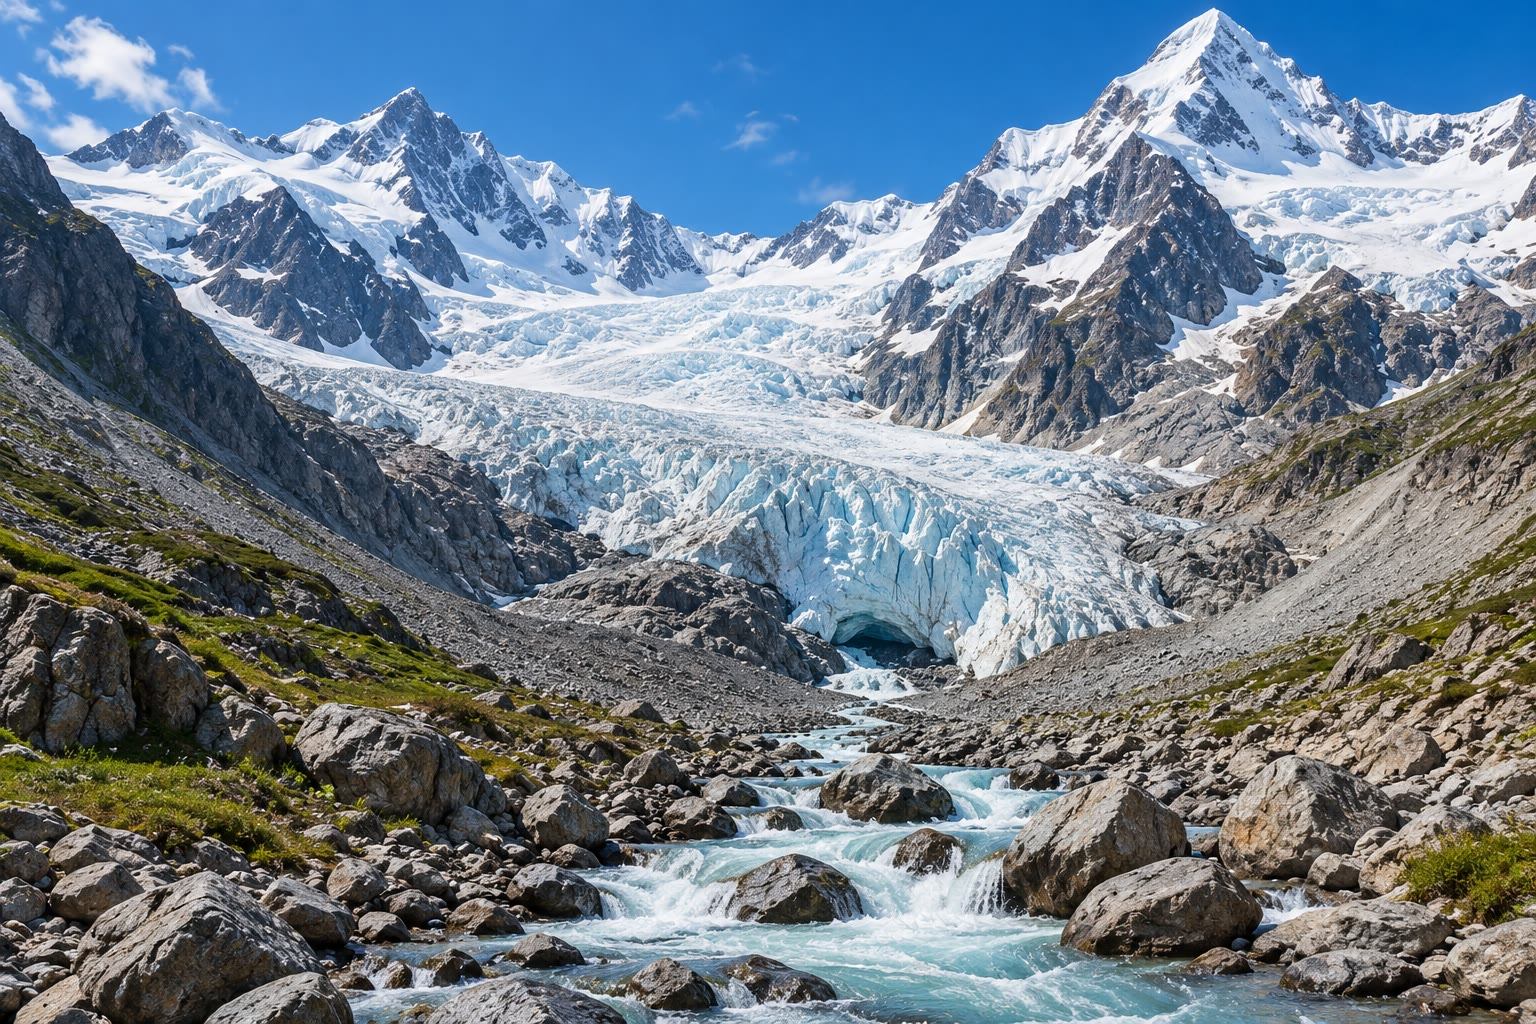
\includegraphics[width=0.62\linewidth]{images/book1/ai/g2-snowy-mountains.jpg}

{\small Les hautes \omterm{def:g1:landscapes-around-us:landform}{montagnes} gardent de l'\omterm{def:g2:water-on-earth:salt-fresh}{eau douce} sous forme de neige et
de glace toute l'année. En été, une partie fond et alimente les torrents.}
\end{omfigure}

Imagine que nous puissions verser toute l'eau de la Terre dans 100 seaux de
la même taille. Combien de seaux chaque sorte d'eau remplirait-elle~?

\begin{omfigure}
\begin{tikzpicture}
  \begin{axis}[hide axis, width=7.2cm, height=7.2cm, xmin=-0.5, xmax=9.5,
      ymin=-0.5, ymax=9.5, axis equal image, scale only axis, clip=false]
    \addplot[scatter, only marks, mark=*, mark size=8pt,
      scatter/classes={0={fill=omSea!80!blue, draw=black!40},
                       1={fill=white, draw=black!60},
                       2={fill=brown!55, draw=black!40}},
      point meta=explicit symbolic]
      table[x=col, y=row, meta=kind] {figdata/out/grade-2-water_shares.dat};
  \end{axis}
  \begin{scope}[shift={(7.9,5.6)}, font=\small]
    \fill[omSea!80!blue, draw=black!40] (0,0) circle (0.2);
    \node[anchor=west] at (0.35,0) {eau salée des océans~: 96 seaux};
    \fill[white, draw=black!60] (0,-0.7) circle (0.2);
    \node[anchor=west] at (0.35,-0.7) {glace et neige~: 2 seaux};
    \fill[brown!55, draw=black!40] (0,-1.4) circle (0.2);
    \node[anchor=west] at (0.35,-1.4) {eau sous la terre~: 2 seaux};
  \end{scope}
\end{tikzpicture}

{\small Toute l'eau de la Terre dans 100 seaux. Les \omterm{def:g1:landscapes-around-us:water}{rivières}, les \omterm{def:g1:landscapes-around-us:water}{lacs}, les
nuages et l'eau de tous les êtres vivants réunis ne rempliraient même pas
un seau. Chiffres du service géologique des États-Unis (USGS).}
\label{fig:g2:water-on-earth:buckets}
\end{omfigure}
% ledger: wss:water-shares (rounded to 100 buckets in figdata/grade-2/water_shares.py)

\begin{proposition}[L'eau de la Terre est surtout salée]\label{prop:g2:water-on-earth:most-salty}
% ledger: wss:water-shares
Sur 100 seaux contenant toute l'eau de la Terre, 96 sont l'\omterm{def:g2:water-on-earth:salt-fresh}{eau salée} des
\omterm{def:g2:water-on-earth:ocean}{océans}. L'\omterm{def:g2:water-on-earth:salt-fresh}{eau douce} que nous buvons n'est qu'une toute petite partie de
toute l'eau~: la plus grande partie est gelée dans les glaces, ou cachée
sous la terre.
\end{proposition}

\section{Où va la pluie~?}

Quand il pleut, l'eau ne reste pas là où elle tombe. Observe la cour de
l'école après une averse~: une partie de l'eau ruisselle sur le sol jusque
dans les caniveaux, une partie s'infiltre dans la terre des
plates-bandes, et les flaques disparaissent lentement quand le soleil
revient.

\begin{omfigure}
\begin{tikzpicture}[x=1cm, y=1cm, font=\small]
  % sky, sea, land
  \fill[ocBlue!6] (0,0) rectangle (12,5.6);
  \fill[omSea] (8.6,0) rectangle (12,0.9);
  \fill[green!30!omLithAlluv] (0,0) -- (0,2.4) .. controls (2,2.6) and (3,2.0) .. (4.5,1.6)
     .. controls (6,1.2) and (7.5,1.0) .. (8.6,0.9) -- (8.6,0) -- cycle;
  % ground below the surface
  \fill[brown!25] (0,0) rectangle (8.6,0.6);
  % river
  \draw[omSea!70!blue, line width=2.4pt] (1.6,2.45) .. controls (3.5,2.0) and (6,1.15) .. (8.6,0.95);
  % cloud and rain
  \pic at (2.2,4.0) {puffycloud};
  \foreach \x in {1.4,1.8,2.2,2.6,3.0}
    \draw[omWxRain, line width=0.8pt] (\x,3.7) -- (\x-0.15,3.1);
  \pic at (9.6,4.3) {puffycloud};
  % arrows
  \draw[omWxRain, line width=1.1pt, -{Stealth[length=2.5mm]}] (3.3,2.15) -- (3.3,0.6);
  \node[anchor=west, align=left, font=\scriptsize] at (3.4,1.0) {une partie\\s'infiltre dans le sol};
  \draw[omWxRain, line width=1.1pt, -{Stealth[length=2.5mm]}] (5.4,1.55) -- (7.6,1.15);
  \node[align=center, font=\scriptsize] at (6.2,2.05) {une partie rejoint une rivière,\\et la rivière va à la mer};
  \draw[black!50, line width=1.1pt, densely dashed, -{Stealth[length=2.5mm]}] (10.2,1.1) .. controls (10.4,2.4) and (10.1,3.2) .. (9.8,3.85);
  \node[align=left, anchor=west, font=\scriptsize] at (10.45,2.4) {l'eau\\s'évapore};
  \draw[black!50, line width=1.1pt, densely dashed, -{Stealth[length=2.5mm]}] (8.45,4.35) -- (3.6,4.3);
  \node[font=\scriptsize, above] at (6.0,4.35) {le vent pousse les nuages};
  \node[font=\scriptsize] at (10.4,0.45) {mer};
  \node[font=\scriptsize, anchor=west] at (0.2,3.25) {pluie};
\end{tikzpicture}

{\small Où va la pluie. L'eau qui monte de la \omterm{def:g2:water-on-earth:ocean}{mer} et des terres sous forme
de vapeur forme de nouveaux nuages, et les nuages apportent une nouvelle
pluie.}
\label{fig:g2:water-on-earth:rain}
\end{omfigure}

\begin{method}[Suivre une goutte de pluie]\label{met:g2:water-on-earth:drop}
Pour suivre une goutte de pluie, pose-toi trois questions, l'une après
l'autre~:
\begin{enumerate}
  \item Où tombe-t-elle~: sur la \omterm{def:g2:water-on-earth:ocean}{mer}, sur un toit, sur le sol, sur une
        \omterm{def:g1:landscapes-around-us:landform}{montagne}~?
  \item S'infiltre-t-elle dans le sol, ruisselle-t-elle à la surface, ou
        gèle-t-elle en glace~?
  \item Où va-t-elle ensuite~: dans une \omterm{def:g1:landscapes-around-us:water}{rivière}, un \omterm{def:g1:landscapes-around-us:water}{lac}, la \omterm{def:g2:water-on-earth:ocean}{mer}, le sol,
        ou de nouveau dans l'air~?
\end{enumerate}
À la fin, chaque goutte revient à la \omterm{def:g2:water-on-earth:ocean}{mer} ou à l'air, et le voyage
recommence.
\end{method}

\begin{example}[Une goutte sur la montagne]\label{ex:g2:water-on-earth:mountain}
Une goutte de pluie tombe en hiver sous forme de neige sur une haute
\omterm{def:g1:landscapes-around-us:landform}{montagne}. Elle y reste, gelée, jusqu'aux journées chaudes de l'été. Alors
elle fond, descend dans un torrent de \omterm{def:g1:landscapes-around-us:landform}{montagne}, rejoint une \omterm{def:g1:landscapes-around-us:water}{rivière}, et la
\omterm{def:g1:landscapes-around-us:water}{rivière} l'emporte jusqu'à la \omterm{def:g2:water-on-earth:ocean}{mer}. Un jour de soleil, la goutte s'évapore
de la \omterm{def:g2:water-on-earth:ocean}{mer} et monte dans l'air, où elle devient une partie d'un nouveau
nuage.
\end{example}

\section{Exercices}

\begin{exercise}[$\star$]\label{exo:g2:water-on-earth:1}
\omterm{def:g2:water-on-earth:salt-fresh}{Eau salée} ou \omterm{def:g2:water-on-earth:salt-fresh}{eau douce}~? La \omterm{def:g2:water-on-earth:ocean}{mer}~; une \omterm{def:g1:landscapes-around-us:water}{rivière}~; la pluie~; un \omterm{def:g1:landscapes-around-us:water}{lac} de
\omterm{def:g1:landscapes-around-us:landform}{montagne}~; un \omterm{def:g2:water-on-earth:ocean}{océan}~; la glace sur une \omterm{def:g1:landscapes-around-us:landform}{montagne}.
\end{exercise}

\begin{exercise}[$\star$]\label{exo:g2:water-on-earth:2}
Pourquoi appelle-t-on la Terre la «~planète bleue~»~?
\end{exercise}

\begin{exercise}[$\star$]\label{exo:g2:water-on-earth:3}
Sur la grille de 100 carrés, 71 carrés sont bleus. Combien de carrés sont
des terres~?
\end{exercise}

\begin{exercise}[$\star$]\label{exo:g2:water-on-earth:4}
Lequel est le plus grand, un \omterm{def:g2:water-on-earth:ocean}{océan} ou une \omterm{def:g2:water-on-earth:ocean}{mer}~?
\end{exercise}

\begin{exercise}[$\star$]\label{exo:g2:water-on-earth:5}
Un marin au milieu de l'\omterm{def:g2:water-on-earth:ocean}{océan} peut-il boire l'eau qui entoure son
bateau~? Pourquoi~?
\end{exercise}

\begin{exercise}[$\star$]\label{exo:g2:water-on-earth:6}
Nomme trois endroits où l'on trouve de l'\omterm{def:g2:water-on-earth:salt-fresh}{eau douce}.
\end{exercise}

\begin{exercise}[$\star\star$]\label{exo:g2:water-on-earth:7}
Sur l'image des 100 seaux, combien de seaux sont de l'\omterm{def:g2:water-on-earth:salt-fresh}{eau salée}~? Combien
sont de l'\omterm{def:g2:water-on-earth:salt-fresh}{eau douce} (la glace et l'eau sous la terre ensemble)~?
\end{exercise}

\begin{exercise}[$\star\star$]\label{exo:g2:water-on-earth:8}
Range dans l'ordre, de ce qui contient le plus d'eau à ce qui en contient
le moins~: les \omterm{def:g1:landscapes-around-us:water}{rivières}~; les \omterm{def:g2:water-on-earth:ocean}{océans}~; la glace et la neige.
\end{exercise}

\begin{exercise}[$\star\star$]\label{exo:g2:water-on-earth:9}
Il pleut sur un champ. Donne deux choses qui peuvent arriver à l'eau.
\end{exercise}

\begin{exercise}[$\star\star$]\label{exo:g2:water-on-earth:10}
Une casserole d'eau de \omterm{def:g2:water-on-earth:ocean}{mer} est laissée au soleil pendant de nombreux
jours, jusqu'à ce que l'eau ait disparu. Que reste-t-il au fond de la
casserole~? Où est partie l'eau~?
\end{exercise}

\begin{exercise}[$\star\star$]\label{exo:g2:water-on-earth:11}
Raconte le voyage d'une goutte de pluie qui tombe sur le toit de l'école,
jusqu'à ce qu'elle soit de nouveau dans un nuage.
\end{exercise}
